\section{Cell Structure and Organization}

\begin{multicols}{2}


%\section*{}


\subsection{Cells, Tissues, Organs} % VSO 22

\begin{center}
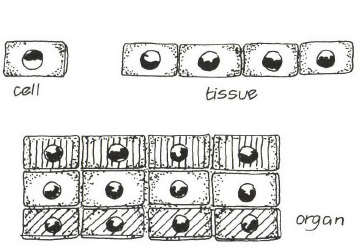
\includegraphics[width=0.49\textwidth]{./img/vso/cells-tissues-organs.jpg}
\end{center}

\begin{description*}
%\item[Subtopic:]{}
\item[Materials:]{Matchboxes, peas/beans/stones, boxes of different colour or size}
%\item[Setup:]{}
\item[Procedure:]{Place a seed in each box. This represents the nucleus: the matchbox the
cell. Place groups of cells inside the coloured boxes - the different
coloured boxes represent different tissues and the boxes themselves
can be joined to make organs.}
%\item[Hazards:]{}
%\item[Questions:]{}
%\item[Observations:]{}
%\item[Theory:]{}
\item[Applications:]{The school is a useful model of an organism. The bricks (cells) make
walls (tissues) and walls make classrooms (organs). The corridors can
therefore be used as models for transport systems.
}
\item[Notes:]{Another analogy might be a town where buildings represent organs,
rooms the tissues or cells and people inside the rooms the various
functions of the cell.}
\end{description*}

\subsection{Cell Models}

\begin{center}
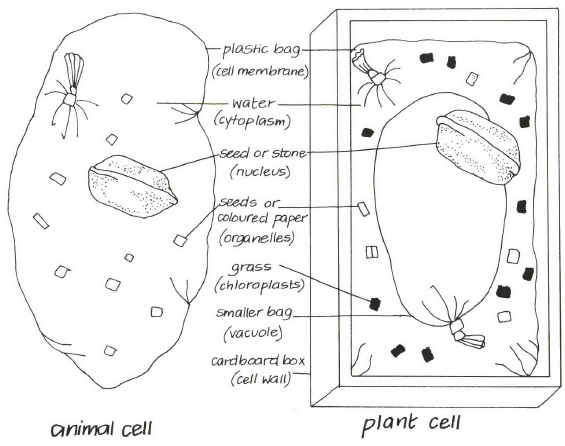
\includegraphics[width=0.49\textwidth]{./img/vso/cell-models.jpg}
\end{center}

\begin{description*}
%\item[Subtopic:]{}
\item[Materials:]{2 large and 2 small plastic bags, water, 2 large seeds/stones, small seeds/coloured paper, grass, cardboard box}
%\item[Setup:]{}
\item[Procedure:]{Make models of plant and animal cells as shown.}
%\item[Hazards:]{}
%\item[Questions:]{}
%\item[Observations:]{}
%\item[Theory:]{}
%\item[Applications:]{}
%\item[Notes:]{}
\end{description*}

\subsection{Looking at Cells} % VSO 23

\begin{center}
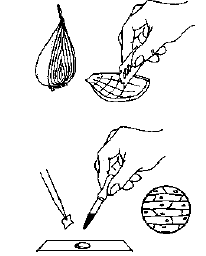
\includegraphics[width=0.35\textwidth]{./img/source/looking-cells.png}
\end{center}

\begin{description*}
%\item[Subtopic:]{}
\item[Materials:]{Onion, pin/needle, glass, plastic strip, iodine solution}
%\item[Setup:]{}
\item[Procedure:]{Cut a slice of onion and gently
peel off a piece of the thin inner
surface skin layer. With a
pin/needle place a piece of `skin'
in a water drop on a piece of
glass. Stain the `skin' with a drop
of iodine solution. Lower a cover
slip (plastic strip) onto the specimen taking care
not to let in any air bubbles.
Now view the prepared
slide through the microscope.}
%\item[Hazards:]{}
%\item[Questions:]{}
%\item[Observations:]{}
%\item[Theory:]{}
%\item[Applications:]{}
%\item[Notes:]{}
\end{description*}

\subsection{How Many Cells?} % VSO 23

%\begin{center}
%\includegraphics[width=0.4\textwidth]{./img/.png}
%\end{center}

\begin{description*}
%\item[Subtopic:]{}
%\item[Materials:]{}
%\item[Setup:]{}
\item[Procedure:]{Ask students to estimate how many cells there are in the human body. How many grains of sand would fit in the human body? Have students make a dot with a sharp pencil.}
%\item[Hazards:]{}
%\item[Questions:]{}
%\item[Observations:]{}
\item[Theory:]{A grain of sand is several thousand times larger than a human cell. Even the largest human cell, the ovum, is smaller than the pencil dot.}
%\item[Applications:]{}
%\item[Notes:]{}
\end{description*}

\columnbreak

\subsection{Simple Microscope} % VSO 23

\begin{center}
%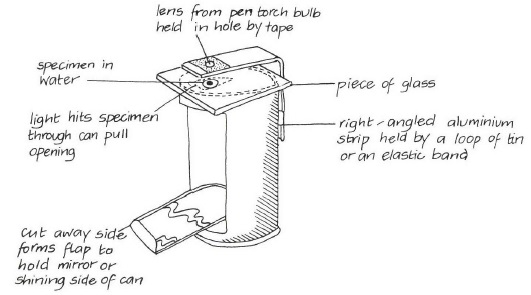
\includegraphics[width=0.49\textwidth]{./img/vso/microscope.jpg}
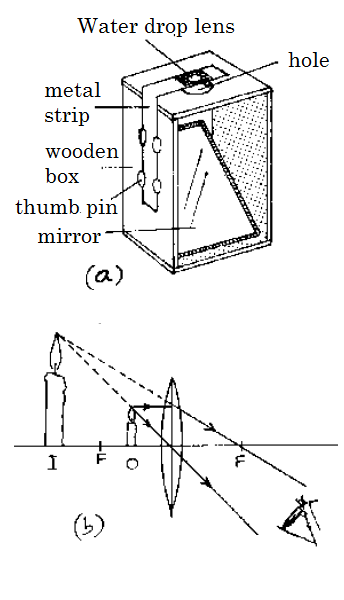
\includegraphics[width=0.49\textwidth]{./img/source/simple-microscope.png}
\end{center}

\begin{description*}
%\item[Subtopic:]{}
\item[Materials:]{Soda can, small lens (e.g. pen-torch bulb), aluminium strip, small mirror, piece of glass, rubber band}
%\item[Setup:]{}
\item[Procedure:]{Make the microscope as shown.
Some care is needed in
positioning the lens in the hole
made for it in the aluminium
strip. The inside of the can may be
painted black. Such a microscope
is quite adequate for looking at
cells.}
%\item[Hazards:]{}
%\item[Questions:]{}
%\item[Observations:]{}
%\item[Theory:]{}
%\item[Applications:]{}
%\item[Notes:]{}
\end{description*}

\vfill
\columnbreak

\subsection{Cell Size}

\begin{center}
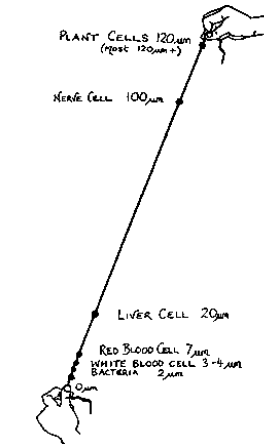
\includegraphics[width=0.4\textwidth]{./img/source/cell-size.png}
\end{center}

\begin{description*}
%\item[Subtopic:]{}
\item[Materials:]{String/chalk}
%\item[Setup:]{}
\item[Procedure:]{Take a piece of string (or chalk a line on the ground) about 60 cm long. Mark distances as
shown in the diagram above. The lengths represent the sizes of different types of cells
enlarged one thousand times.}
%\item[Hazards:]{}
\item[Questions:]{How many times bigger is a plant stem cell than a blood cell?}
\item[Observations:]{50 times.}
\item[Theory:]{Although almost all cells are too small to be seen with the unaided eye, they show a wide
range of sizes (about the same range as a mouse and an elephant).}
%\item[Applications:]{}
%\item[Notes:]{}
\end{description*}

%==================================================================================================%


\end{multicols}

\pagebreak